% Standalone, anonymized Methods and Results report for the dual-fitness audit.
\documentclass[sn-mathphys-num,Numbered]{sn-jnl}

\usepackage{amsmath,amssymb,bm}
\usepackage{booktabs}
\usepackage{tabularx}
\usepackage{graphicx}
\usepackage{hyperref}

\renewcommand{\topfraction}{0.95}
\renewcommand{\bottomfraction}{0.85}
\renewcommand{\textfraction}{0.05}
\renewcommand{\floatpagefraction}{0.75}

\begin{document}

\title{Dual-Fitness Optimizer Benchmark for Neural Intraday Trend Classification: Methodology and Results}
\maketitle

\section{Materials and Methods}

\subsection{Study Design and Data Partitioning}

This report evaluates whether the \emph{selection objective} used by an optimizer changes the out-of-sample behaviour of neural and machine-learning classifiers. The data comprise 15,057 chronologically ordered 5-minute bars from B3 Mini-Index futures, obtained from the BovDB collection \cite{cardoso2022bovdb,souza2024dataset}. Seven technical indicators were retained by Information Gain screening. All experiments use the same sequential 60/20/20 train/validation/test split, with 9,034 training bars, 3,011 validation bars, and 3,012 locked test bars. No shuffling is performed.

Figure~\ref{fig:dual_workflow} makes the experimental comparison explicit. The data, features, model families, optimizer families, and evaluation budget are shared; only the validation fitness changes. The test set remains unavailable during both optimization procedures.

\begin{figure}[htbp]
\centering
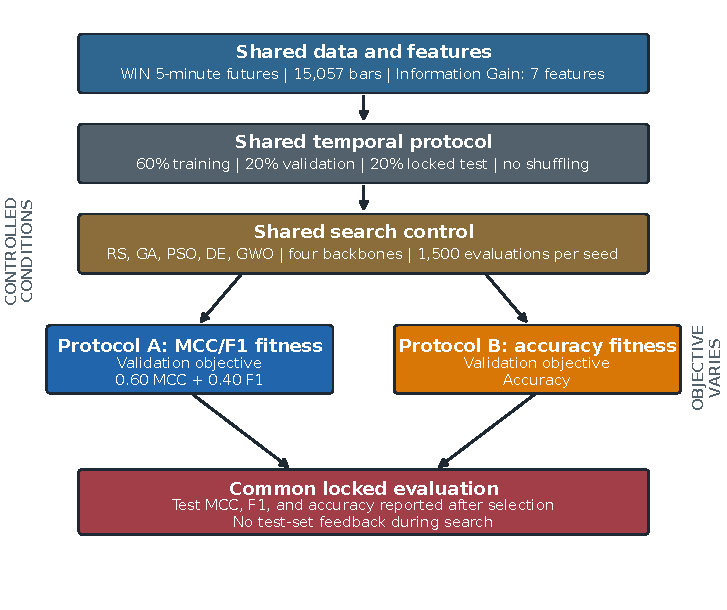
\includegraphics[width=0.93\linewidth]{figures/dual_fitness_protocol_overview.pdf}
\caption{Controlled comparison of two optimization protocols. Shared conditions are held fixed; the validation objective alone varies. Both protocols are evaluated once on the same locked test block after model selection.}
\label{fig:dual_workflow}
\end{figure}

\begin{figure}[htbp]
\centering
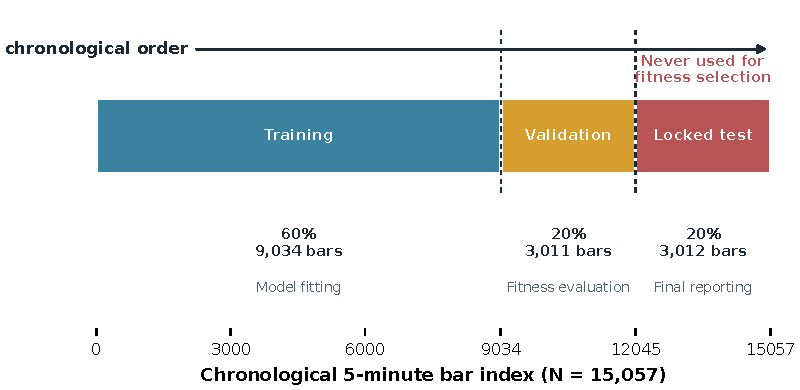
\includegraphics[width=0.88\linewidth]{figures/dual_fitness_temporal_split.pdf}
\caption{Chronological train/validation/test partition used by both protocols. The test block is never used for fitness evaluation or hyperparameter selection.}
\label{fig:dual_split}
\end{figure}

\subsection{Shared Search Controls}

Four model backbones (MLP, Random Forest, SVM, and 1D-CNN) are optimized by Random Search (RS), Genetic Algorithm (GA), Particle Swarm Optimization (PSO), Differential Evolution (DE), and Grey Wolf Optimizer (GWO). Each model--optimizer--protocol combination is given the same cap of $N_{\mathrm{eval}}=1{,}500$ candidate evaluations per seed. This equal-budget condition prevents an optimizer from obtaining an apparent advantage merely by evaluating more candidates.

\subsection{Two Validation Fitness Functions}

Protocol A selects candidate configurations using a compound validation objective designed to emphasize imbalance-robust discrimination:
\begin{equation}
f_{\mathrm{MCC/F1}}(\boldsymbol{\theta})=0.60\,\mathrm{MCC}_{\mathrm{val}}(\boldsymbol{\theta})+0.40\,F_{1,\mathrm{val}}(\boldsymbol{\theta}).
\end{equation}

Protocol B uses the conventional validation-accuracy objective:
\begin{equation}
f_{\mathrm{Acc}}(\boldsymbol{\theta})=\mathrm{Accuracy}_{\mathrm{val}}(\boldsymbol{\theta}).
\end{equation}

The objective is used solely to rank candidate configurations on the validation block. After selection, both protocols report test accuracy, test MCC, and test $F_1$. Consequently, test accuracy under Protocol A is a secondary outcome of MCC/F1-directed selection, whereas test accuracy under Protocol B is the primary outcome of accuracy-directed selection. This distinction is essential: a reported metric and the fitness that generated the selected model are not interchangeable.

\subsection{Available Evidence and Reporting Scope}

The audit uses the three paired seeds available in both protocols (seeds 1--3) for every one of the 20 model--optimizer cells, yielding 60 seed-level observations per protocol. Results are therefore descriptive: figures display configuration means across the three matched seeds and their search trajectories. No Friedman, Wilcoxon, Holm-adjusted $p$-values, or standardized effect sizes are claimed in this report. Confirmatory inference requires a prespecified rerun with at least 20 common seeds per cell.

\section{Results}

\subsection{Objective-Dependent Out-of-Sample Performance}

Figure~\ref{fig:paired_outcomes} displays the held-out outcomes for each of the 20 model--optimizer cells. Across these cells, the unweighted macro mean test accuracy was 0.623 for MCC/F1 fitness and 0.617 for accuracy fitness. The corresponding macro mean test MCC values were 0.247 and 0.235, respectively. These values are descriptive averages of cell-level means, not population estimates.

The paired display is more informative than a single aggregate bar: it shows that the effect of the objective varies across configurations. Accuracy-directed selection does not uniformly increase held-out accuracy in the currently available runs, and its effect on MCC is likewise backbone- and optimizer-dependent. This is precisely the empirical question that the dual-fitness design makes testable once the confirmatory seed budget is complete.

\begin{figure}[htbp]
\centering
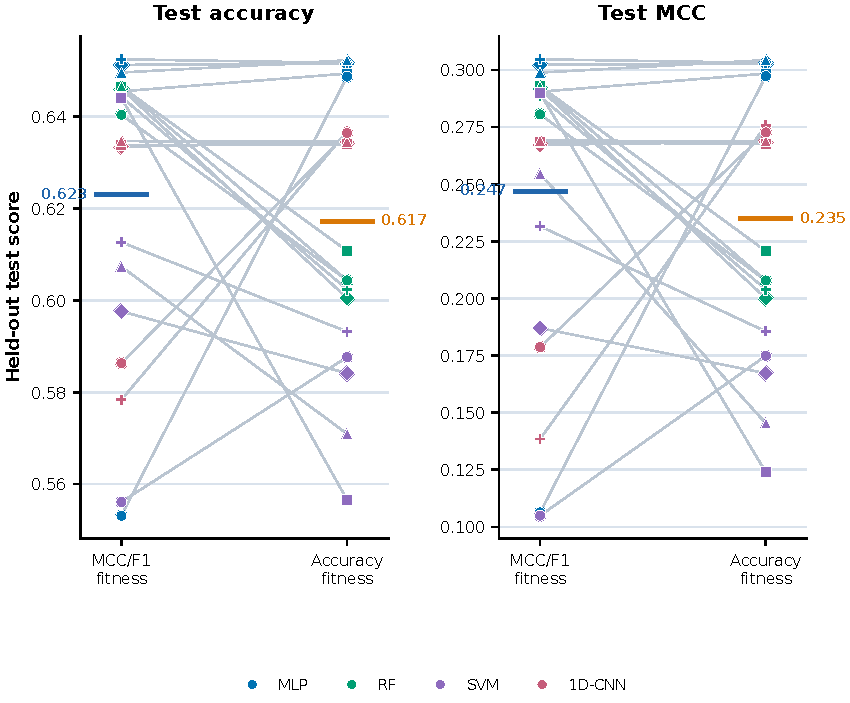
\includegraphics[width=0.96\linewidth]{figures/dual_fitness_paired_outcomes.pdf}
\caption{Held-out performance under the two validation objectives. Each connected pair is the mean of the same three seeds for one model--optimizer cell; colour identifies the backbone and marker shape identifies the optimizer. Short horizontal segments give the macro mean across the 20 cells.}
\label{fig:paired_outcomes}
\end{figure}

\subsection{Where the Objective Changes Performance}

Figure~\ref{fig:delta_heatmaps} resolves the protocol contrast by backbone and optimizer. Each cell reports the signed difference between the accuracy-fitness and MCC/F1-fitness protocols. Positive values favour accuracy fitness and negative values favour MCC/F1 fitness. The pattern is heterogeneous rather than universal, which precludes a defensible claim that either objective is globally superior on the present three-seed evidence.

\begin{figure}[htbp]
\centering
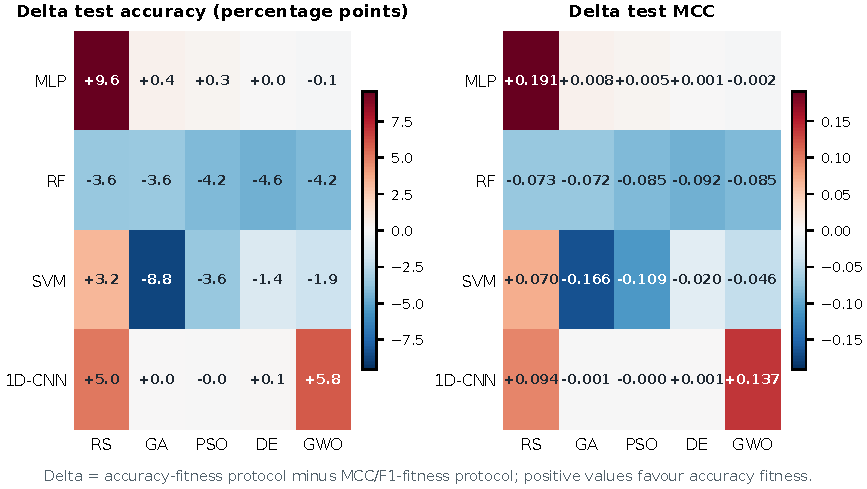
\includegraphics[width=0.98\linewidth]{figures/dual_fitness_delta_heatmaps.pdf}
\caption{Configuration-level change in held-out metrics induced by the validation objective. Values are accuracy-fitness minus MCC/F1-fitness means over the paired seeds 1--3. The left panel uses percentage points; the right panel uses raw MCC units.}
\label{fig:delta_heatmaps}
\end{figure}

\subsection{Convergence Under the Two Objectives}

Figure~\ref{fig:dual_convergence} shows search dynamics for the MLP reference backbone. The left panel tracks the compound MCC/F1 validation fitness, whereas the right panel tracks validation accuracy. These curves must not be interpreted on a common vertical scale: they represent different objectives. Their role is to show how each optimizer progresses under the criterion it was assigned, not to establish cross-protocol statistical superiority.

\begin{figure}[htbp]
\centering
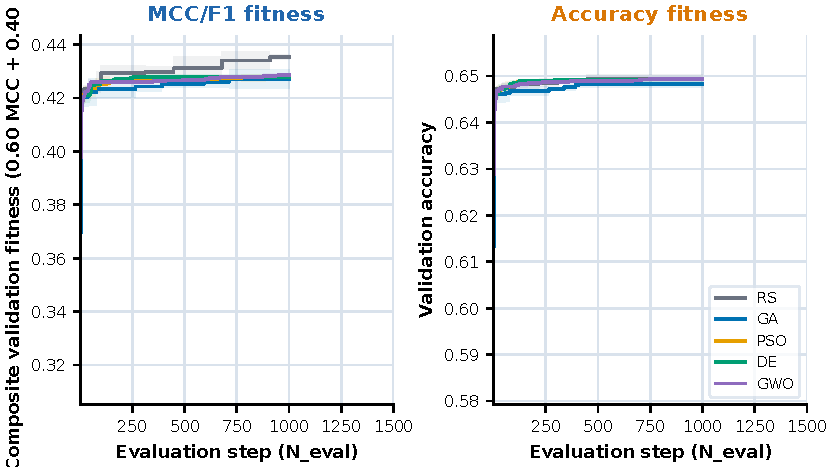
\includegraphics[width=0.98\linewidth]{figures/dual_fitness_convergence.pdf}
\caption{Convergence trajectories for the MLP reference backbone under the two validation objectives. Solid lines are means and shaded ribbons are $\pm1$ standard deviation across the three paired seeds. Left: composite MCC/F1 validation fitness. Right: validation accuracy.}
\label{fig:dual_convergence}
\end{figure}

\subsection{Interpretation and Confirmatory Next Step}

The present results establish a controlled, visually auditable comparison between two fitness functions, but they do not yet support confirmatory ranking claims. The next experimental stage should complete a common 20-seed design for every model--optimizer cell, retain the same temporal split and budget, and apply a prespecified paired analysis separately for test MCC and test accuracy. Only then should omnibus and post-hoc tests be used to quantify objective-specific advantages.

\bibliography{references}

\end{document}
